\documentclass{article}

% ---------------------------------------------------------
% 1. SETUP & PACKAGES
% ---------------------------------------------------------
\PassOptionsToPackage{numbers, compress}{natbib}

% [preprint] shows your names. Change to [final] for the final version.
\usepackage[final]{neurips_2024}

% Remove the conference footer from the first page
\makeatletter
\renewcommand{\@noticestring}{}
\makeatother

\usepackage[utf8]{inputenc} % allow utf-8 input
\usepackage[T1]{fontenc}    % use 8-bit T1 fonts
\usepackage[french, provide=*]{babel}  % French language support
\usepackage{hyperref}       % hyperlinks
\usepackage{url}            % simple URL typesetting
\usepackage{booktabs}       % professional-quality tables
\usepackage{amsmath}        % best math environment
\usepackage{amsthm}         % for theorems
\newtheorem{theorem}{Théorème}
\usepackage{amsfonts}       % blackboard math symbols
\usepackage{nicefrac}       % compact symbols for 1/2, etc.
\usepackage[expansion=false]{microtype}      % microtypography
\usepackage{graphicx}       % for images
\usepackage{enumitem}       % for cleaner lists
\usepackage{multirow}
\usepackage{xcolor}         % color text
\usepackage{tikz}
\usetikzlibrary{shapes.geometric, arrows.meta, positioning, calc, decorations.pathreplacing}
\usepackage{pgfplots}
\usepackage{float}
\usepackage{natbib}
\pgfplotsset{compat=1.18}

% Custom Colors
\definecolor{myBlue}{RGB}{70, 130, 180}
\definecolor{myOrange}{RGB}{255, 140, 0}
\definecolor{myGreen}{RGB}{60, 179, 113}


% ---------------------------------------------------------
% 2. TITLE & AUTHORS
% ---------------------------------------------------------
\title{IWAE vs VAE : Borne Plus Serrée, Latents Plus Riches ?}

\author{%
  Amine Mike El Maalouf \\
  \texttt{amine.el-maalouf@epita.fr} \\
  \And
  Cedric Damais \\
  \texttt{cedric.damais@epita.fr} \\
  \And
  Yacine Benihaddadene \\
  \texttt{yacine.benihaddadene@epita.fr} \\
  \And
  Leon Ayral \\
  \texttt{leon.ayral@epita.fr} \\
  \And
  Oscar Le Dauphin \\
  \texttt{oscar.le-dauphin@epita.fr} \\
}

\begin{document}

\maketitle

% ---------------------------------------------------------
% 3. ABSTRACT
% ---------------------------------------------------------

\begin{abstract}
Les Autoencodeurs Variationnels (VAE) sont des modèles génératifs permettant
d'approximer des distributions a posteriori complexes via la maximisation d'une
borne inférieure variationnelle (ELBO). Cependant, l'objectif standard du VAE
contraint souvent le modèle à apprendre des représentations simplifiées,
limitant ainsi sa capacité de modélisation. Ce projet étudie l'Importance
Weighted Autoencoder (IWAE), une généralisation du VAE qui optimise une borne
strictement plus fine dérivée de l'échantillonnage préférentiel. Nous analysons
l'impact théorique de cet objectif sur l'estimation des gradients et la
flexibilité du postérieur. Nos expériences sur le jeu de données MNIST
démontrent que l'utilisation de multiples échantillons pondérés ($K>1$) améliore
significativement la log-vraisemblance par rapport au VAE standard ($K=1$). De
plus, nos résultats confirment que l'IWAE exploite plus efficacement l'espace
latent, augmentant le nombre d'unités actives et produisant des représentations
plus riches. Cependant, nous étudions également une limitation critique :
lorsque $K$ augmente, le rapport signal sur bruit (SNR) des gradients de
l'encodeur diminue, dégradant potentiellement la capacité d'apprentissage de
celui-ci.
\end{abstract}

\newpage
% ---------------------------------------------------------
% 4. SECTIONS
% ---------------------------------------------------------
\section{Introduction}

Les modèles génératifs profonds sont devenus un pilier de l'apprentissage
automatique moderne, permettant la synthèse de données complexes telles que des
images, du texte et de l'audio. Parmi ceux-ci, l'Autoencodeur Variationnel (VAE)
\cite{kingma2013auto} se distingue comme une approche rigoureuse combinant
réseaux de neurones et inférence bayésienne. En apprenant une correspondance
probabiliste entre les observations et un espace latent structuré, les VAE
offrent un cadre puissant pour la génération et l'apprentissage de
représentations.

Cependant, l'objectif standard du VAE présente des limitations inhérentes. La
borne inférieure sur l'évidence (ELBO) que les VAE maximisent peut être une
approximation lâche de la vraie log-vraisemblance lorsque le postérieur approché
$q_\phi(z|x)$ ne parvient pas à correspondre au vrai postérieur $p_\theta(z|x)$.
Ce relâchement conduit à des phénomènes tels que l'effondrement du postérieur
(posterior collapse), où le modèle ignore les dimensions latentes informatives
et s'appuie entièrement sur le décodeur.

L'Importance Weighted Autoencoder (IWAE), introduit par
\citet{burda2015importance}, répond à cette limitation en utilisant
l'échantillonnage préférentiel pour obtenir une borne strictement plus serrée
sur la log-vraisemblance. Dans ce rapport, nous étudions les fondements
théoriques de l'IWAE, comparons ses performances au VAE standard sur le jeu de
données MNIST, et explorons à la fois ses avantages et ses inconvénients
potentiels. Nous examinons également les développements récents de la recherche
qui ont construit sur le cadre de l'IWAE.

% ---------------------------------------------------------
\section{Contexte Théorique}

\subsection{Le Paradigme des Modèles à Variables Latentes}

L'apprentissage profond génératif repose sur l'hypothèse fondamentale que les données de haute dimension que nous observons (par exemple, des images ou du son) ne sont pas uniformément réparties dans l'espace d'entrée, mais résident sur des variétés de dimension inférieure.

Soit $\mathcal{D} = \{x^{(i)}\}_{i=1}^N$ un ensemble de données i.i.d. de variable $x \in \mathcal{X}$. Nous supposons que ces données sont générées par un processus aléatoire non observé impliquant une variable latente continue $z \in \mathcal{Z}$, où typiquement $\text{dim}(z) \ll \text{dim}(x)$. Le processus génératif est défini par la factorisation conjointe :
\begin{equation}
    p_\theta(x, z) = p_\theta(x|z)p(z)
\end{equation}

Ici, $p(z)$ est la distribution a priori (prior), souvent fixée comme une normale standard multivariée $\mathcal{N}(0, I)$, et $p_\theta(x|z)$ est la distribution de vraisemblance (likelihood), modélisée par un réseau de neurones paramétré par $\theta$ (le décodeur). Ce réseau apprend une transformation non linéaire complexe permettant de passer de l'espace latent abstrait à l'espace des données observables.

\subsection{Le Problème de l'Intractabilité}

L'objectif central de l'inférence bayésienne est de calculer la distribution a posteriori des variables latentes étant donné une observation, notée $p_\theta(z|x)$. Selon la règle de Bayes :
\begin{equation}
    p_\theta(z|x) = \frac{p_\theta(x|z)p(z)}{p_\theta(x)}
\end{equation}

Le terme au dénominateur, $p_\theta(x)$, est l'évidence marginale (ou vraisemblance marginale). Elle s'obtient par marginalisation de la variable latente $z$ :
\begin{equation}
    p_\theta(x) = \int p_\theta(x|z)p(z) \, dz
\end{equation}

Or on a arrive pas à calculer analytiquement cette intégrale dans la plupart des cas, car le modèle génératif $p_\theta(x|z)$ est souvent non linéaire et complexe.

Cette intractabilité de $p_\theta(x)$ rend le calcul direct du postérior $p_\theta(z|x)$ impossible, nécessitant le recours à des méthodes d'approximation.

\subsection{Inférence Variationnelle (VI)}

Pour contourner l'intractabilité du postérior vrai, l'Inférence Variationnelle propose de l'approcher par une distribution paramétrique $q_\phi(z|x)$, appelée \textit{distribution variationnelle} (ou encodeur), paramétrée par $\phi$.
L'objectif est de trouver les paramètres $\phi$ qui minimisent la divergence entre l'approximation et la vraie distribution. La métrique standard utilisée est la divergence de Kullback-Leibler (KL) :

\begin{equation}
    \mathbb{KL}(q_\phi(z|x) || p_\theta(z|x)) = \mathbb{E}_{z \sim q_\phi} \left[ \log \frac{q_\phi(z|x)}{p_\theta(z|x)} \right]
\end{equation}

Cependant, minimiser directement cette KL divergence est impossible car elle dépend du terme inconnu $p_\theta(z|x)$.

\subsection{La Borne Inférieure de l'Évidence (ELBO)}

Nous pouvons reformuler le problème en analysant la log-vraisemblance marginale. En utilisant les propriétés du logarithme et de l'espérance, nous avons :
\begin{equation}
    \log p_\theta(x) = \mathbb{E}_{z \sim q_\phi} [\log p_\theta(x)] = \mathbb{E}_{z \sim q_\phi} \left[ \log \frac{p_\theta(x, z)}{p_\theta(z|x)} \right]
\end{equation}

En multipliant et divisant par $q_\phi(z|x)$ à l'intérieur du logarithme, nous obtenons la décomposition fondamentale suivante :
\begin{align}
    \log p_\theta(x) &= \mathbb{E}_{q_\phi} \left[ \log \frac{p_\theta(x, z)}{q_\phi(z|x)} \frac{q_\phi(z|x)}{p_\theta(z|x)} \right] \\
    &= \underbrace{\mathbb{E}_{q_\phi} \left[ \log \frac{p_\theta(x, z)}{q_\phi(z|x)} \right]}_{\mathcal{L}_{\text{ELBO}}(\theta, \phi; x)} + \underbrace{\mathbb{KL}(q_\phi(z|x) || p_\theta(z|x))}_{\ge 0}
\end{align}

Puisque la divergence KL est toujours positive ou nulle, le terme $\mathcal{L}_{\text{ELBO}}$ constitue une borne inférieure stricte sur la log-vraisemblance des données :
\begin{equation}
    \log p_\theta(x) \ge \mathcal{L}_{\text{ELBO}}(\theta, \phi; x)
\end{equation}

Dans le cadre du VAE standard, cette borne est maximisée par descente de gradient stochastique. L'ELBO peut être réécrite sous une forme plus intuitive :
\begin{equation}
    \mathcal{L}_{\text{ELBO}} = \mathbb{E}_{q_\phi(z|x)} [\log p_\theta(x|z)] - \mathbb{KL}(q_\phi(z|x) || p(z))
\end{equation}
Le premier terme encourage une reconstruction fidèle des données (minimisation de l'erreur de reconstruction), tandis que le second agit comme un régularisateur, forçant la distribution latente apprise $q_\phi$ à rester proche du prior $p(z)$.
\subsection{VAE Standard : L'Objectif ELBO}

Le VAE maximise la borne inférieure sur l'évidence (ELBO), qui fournit une borne inférieure sur la log-vraisemblance :
\begin{equation}
    \log p_\theta(x) \geq \mathcal{L}_{\text{VAE}} = \mathbb{E}_{z \sim q_\phi(z|x)} \left[ \log \frac{p_\theta(x,z)}{q_\phi(z|x)} \right]
\end{equation}

Cette borne peut être décomposée en :
\begin{equation}
    \mathcal{L}_{\text{VAE}} = \mathbb{E}_{q_\phi(z|x)}[\log p_\theta(x|z)] - \text{KL}(q_\phi(z|x) \| p(z))
\end{equation}

L'écart entre la vraie log-vraisemblance et l'ELBO est précisément la divergence KL entre les postérieurs approché et vrai :
\begin{equation}
    \log p_\theta(x) - \mathcal{L}_{\text{VAE}} = \text{KL}(q_\phi(z|x) \| p_\theta(z|x))
\end{equation}

Lorsque le postérieur approché $q_\phi(z|x)$ est trop simple (par exemple, une gaussienne diagonale) pour capturer le vrai postérieur, la borne devient lâche. Ce relâchement contribue au risque d'\textbf{effondrement du postérieur}, où le terme KL domine et le modèle apprend à ignorer le code latent.

% ---------------------------------------------------------
\section{La Solution IWAE}

L'Importance Weighted Autoencoder (IWAE) \cite{burda2015importance} ne se contente pas d'être une simple extension du VAE ; il représente un pont fondamental entre l'Inférence Variationnelle (VI) et les méthodes de Monte Carlo (Importance Sampling). Il répond au relâchement de la borne ELBO en exploitant la capacité de l'échantillonnage préférentiel à corriger les inadéquations entre la distribution variationnelle $q_\phi$ et le vrai postérior.

\subsection{L'Objectif IWAE : Une Perspective Monte Carlo}

L'objectif IWAE est défini par l'espérance logarithmique de la moyenne de $K$ rapports de densité. Contrairement au VAE qui utilise $K=1$, l'IWAE construit un estimateur de la vraisemblance marginale $p_\theta(x)$ :

\begin{equation}
    \mathcal{L}_K(x) = \mathbb{E}_{z_1, \ldots, z_K \sim q_\phi(z|x)} \left[ \log \left( \frac{1}{K} \sum_{i=1}^{K} w_i \right) \right]
\end{equation}

où les \textit{poids d'importance non normalisés} sont définis par le rapport :
\begin{equation}
    w_i = \frac{p_\theta(x, z_i)}{q_\phi(z_i|x)}
\end{equation}

Intuitivement, $\frac{1}{K} \sum w_i$ est un estimateur non biaisé de $p_\theta(x)$. Cependant, comme nous optimisons le logarithme de cette quantité (pour la stabilité numérique et la compatibilité avec les réseaux de neurones), l'estimateur devient biaisé en raison de l'inégalité de Jensen ($\mathbb{E}[\log X] \le \log \mathbb{E}[X]$). L'IWAE cherche à réduire ce biais en augmentant $K$.

\subsection{Nouveauté 1 : Bornes Strictement Plus Serrées}

La contribution théorique majeure de \cite{burda2015importance} est la preuve que l'augmentation du nombre d'échantillons $K$ resserre strictement la borne inférieure.

\begin{theorem}[Monotonie de la Borne]
Pour tout $K \ge 1$, la borne IWAE $\mathcal{L}_K$ est minorée par $\mathcal{L}_{K-1}$ et majorée par la log-vraisemblance réelle :
\begin{equation}
    \mathcal{L}_1 \leq \mathcal{L}_2 \leq \cdots \leq \mathcal{L}_K \leq \log p_\theta(x)
\end{equation}
\end{theorem}

Cela implique que l'IWAE permet d'échanger de la puissance de calcul (plus de $K$) contre une meilleure approximation de la log-vraisemblance, sans changer l'architecture du modèle.

\subsubsection{Démonstration : Borne monotonement croissante}

Nous présentons ici une preuve formalisée utilisant la technique du sous-ensemble.

Soit un ensemble d'indices $S_K = \{1, \dots, K\}$. Considérons un sous-ensemble $I \subset S_K$ de taille $m < K$, choisi uniformément.
Nous utilisons l'observation suivante sur les moyennes empiriques :
\begin{equation}
    \frac{1}{K} \sum_{i=1}^K w_i = \mathbb{E}_{I} \left[ \frac{1}{m} \sum_{j \in I} w_j \right]
\end{equation}
où l'espérance $\mathbb{E}_I$ porte sur le choix aléatoire du sous-ensemble $I$.

En substituant cette égalité dans la définition de $\mathcal{L}_K$ et en appliquant l'inégalité de Jensen (la fonction logarithme étant concave) :

\begin{align}
\mathcal{L}_k &= \mathbb{E}_{\mathbf{h}_1, \dots, \mathbf{h}_k} \left[ \log \frac{1}{k} \sum_{i=1}^k \frac{p(\mathbf{x}, \mathbf{h}_i)}{q(\mathbf{h}_i|\mathbf{x})} \right] \tag{17} \\
&= \mathbb{E}_{\mathbf{h}_1, \dots, \mathbf{h}_k} \left[ \log \mathbb{E}_{I=\{i_1, \dots, i_m\}} \left[ \frac{1}{m} \sum_{j=1}^m \frac{p(\mathbf{x}, \mathbf{h}_{i_j})}{q(\mathbf{h}_{i_j}|\mathbf{x})} \right] \right] \tag{18} \\
&\geq \mathbb{E}_{\mathbf{h}_1, \dots, \mathbf{h}_k} \left[ \mathbb{E}_{I=\{i_1, \dots, i_m\}} \left[ \log \frac{1}{m} \sum_{j=1}^m \frac{p(\mathbf{x}, \mathbf{h}_{i_j})}{q(\mathbf{h}_{i_j}|\mathbf{x})} \right] \right] \tag{19} \\
&= \mathbb{E}_{\mathbf{h}_1, \dots, \mathbf{h}_m} \left[ \log \frac{1}{m} \sum_{i=1}^m \frac{p(\mathbf{x}, \mathbf{h}_i)}{q(\mathbf{h}_i|\mathbf{x})} \right] = \mathcal{L}_m \tag{20}
\end{align}

Puisque les échantillons $z_i$ sont i.i.d., l'espérance interne ne dépend que de $m$ échantillons, ce qui est exactement la définition de $\mathcal{L}_m$. Ainsi, $\mathcal{L}_K \ge \mathcal{L}_m$.

\subsection{Nouveauté 2 : Le Postérieur Implicite et les Gradients}

Contrairement au VAE qui force le postérior $q_\phi(z|x)$ à correspondre au vrai postérior $p_\theta(z|x)$ (souvent unimodal et gaussien), l'IWAE introduit une distribution plus flexible appelée \textit{postérior corrigé par l'importance} (Importance Weighted Posterior).

\subsubsection{Les Poids Normalisés comme Filtre}
Définissons les poids d'importance normalisés $\tilde{w}_i$ :
\begin{equation}
    \tilde{w}_i = \frac{w_i}{\sum_{j=1}^K w_j}, \quad \text{avec } \sum_{i=1}^K \tilde{w}_i = 1
\end{equation}

Ces poids quantifient la qualité relative de chaque échantillon.

Si $z_i$ est un "mauvais" échantillon (faible $p(x|z)$), alors $\tilde{w}_i \to 0$. Si $z_i$ est proche de la vraie distribution latente, $\tilde{w}_i$ domine.

L'approximation implicite du postérior par l'IWAE, notée $q_{EW}(z|x)$, converge vers le vrai postérior lorsque $K \to \infty$ :
\begin{equation}
    q_{EW}(z|x) \approx \sum_{i=1}^K \tilde{w}_i \delta(z - z_i) \xrightarrow{K \to \infty} p_\theta(z|x)
\end{equation}

\subsubsection{Analyse du Gradient}
L'impact de ce mécanisme est visible dans le calcul du gradient pour l'encodeur $\phi$. En utilisant l'astuce de reparamétrisation ($z_i = \mu + \sigma \odot \epsilon_i$), le gradient devient :

\begin{equation}
    \nabla_\phi \mathcal{L}_K = \mathbb{E}_{\epsilon_{1:K}} \left[ \sum_{i=1}^{K} \tilde{w}_i \nabla_\phi \log w(x, z_i(\phi)) \right]
\end{equation}

Cette équation révèle une différence cruciale avec le VAE :
\begin{itemize}
    \item Dans un \textbf{VAE} ($K=1$), $\tilde{w}_1 = 1$. Le gradient est calculé sur l'échantillon, qu'il soit bon ou mauvais.
    \item Dans un \textbf{IWAE} ($K>1$), le terme $\tilde{w}_i$ agit comme une pondération automatique. Les gradients provenant de "mauvais" échantillons sont multipliés par un poids proche de 0 et sont donc ignorés. Le modèle apprend principalement des échantillons qui expliquent bien les données.
\end{itemize}

\subsection{Interprétation : Le Filet de Sécurité}

L'intuition clé derrière la robustesse de l'IWAE peut être vue comme un effet de "filet de sécurité" (Safety Net).

Dans un VAE standard, si l'encodeur échantillonne une valeur $z$ très improbable (dans les queues de distribution), le terme $\log p(x|z)$ devient extrêmement négatif, causant une variance massive dans les gradients.

Avec l'IWAE, tant qu'au moins \textit{un} des $K$ échantillons tombe dans une région de haute probabilité, la moyenne $\sum w_i$ reste stable. Mathématiquement, la somme à l'intérieur du logarithme empêche l'effondrement vers $-\infty$ :
\begin{equation}
    \log(w_{\text{mauvais}} + w_{\text{bon}}) \approx \log(w_{\text{bon}}) \gg \log(w_{\text{mauvais}})
\end{equation}

Cela permet à l'encodeur d'explorer l'espace latent avec moins de risque, favorisant une couverture plus large des modes de la distribution (Mode Covering) plutôt que de se concentrer sur un seul mode (Mode Seeking) comme le fait souvent la divergence KL standard.
\subsection{Le Paradoxe du SNR}

Lorsque $K \to \infty$, quelque chose de contre-intuitif se produit. Considérons les poids normalisés $\tilde{w}_i$ :

\begin{itemize}
    \item À mesure que $K$ augmente, la distribution des poids d'importance devient plus concentrée : typiquement un échantillon aura $\tilde{w}_i \approx 1$ tandis que tous les autres auront $\tilde{w}_j \approx 0$.
    \item La mise à jour du gradient est dominée par le seul échantillon ``gagnant''.
    \item Cet échantillon gagnant est de plus en plus déterminé par l'a priori $p(z)$ et la vraisemblance $p_\theta(x|z)$, et non par la qualité de l'encodeur $q_\phi(z|x)$.
\end{itemize}

Mathématiquement, lorsque $K \to \infty$, l'objectif IWAE approche :
\begin{equation}
    \mathcal{L}_\infty = \log p_\theta(x) = \log \mathbb{E}_{z \sim q_\phi}[w(x, z)]
\end{equation}

À cette limite, l'objectif dépend de l'encodeur uniquement à travers son support, pas sa distribution spécifique. Tant que $q_\phi(z|x) > 0$ partout où $p_\theta(x,z) > 0$, la borne est exacte. Cela signifie que le signal de gradient pour $\phi$ disparaît.

\subsection{Analyse du Rapport Signal sur Bruit}

Le SNR du gradient de l'encodeur peut être défini comme :
\begin{equation}
    \text{SNR}(\nabla_\phi \mathcal{L}_K) = \frac{|\mathbb{E}[\nabla_\phi \mathcal{L}_K]|}{\text{Std}[\nabla_\phi \mathcal{L}_K]}
\end{equation}

\citet{rainforth2018tighter} ont montré que tandis que le SNR pour le décodeur $\theta$ augmente avec $K$, le SNR pour l'encodeur $\phi$ diminue avec $K$ :
\begin{equation}
    \text{SNR}(\nabla_\phi \mathcal{L}_K) = \mathcal{O}(K^{-1/2})
\end{equation}

Cela signifie que bien que nous obtenions une meilleure estimation de la log-vraisemblance, l'encodeur reçoit des signaux de gradient de plus en plus bruités et faibles.

\subsection{Implications Pratiques}

Cette dégradation du SNR a des conséquences importantes :
\begin{itemize}
    \item \textbf{Le décodeur apprend bien :} Le modèle génératif $p_\theta(x|z)$ continue de s'améliorer avec un $K$ plus grand.
    \item \textbf{L'encodeur peut stagner :} Le réseau d'inférence $q_\phi(z|x)$ reçoit des signaux de gradient diminuants et peut échouer à s'améliorer.
\end{itemize}

Cette analyse suggère que simplement augmenter $K$ n'est pas toujours bénéfique. L'objectif IWAE crée une asymétrie où le décodeur bénéficie de plus d'échantillons tandis que l'encodeur en souffre.

% ---------------------------------------------------------
\section{Méthodologie Expérimentale}

Cette section détaille le protocole expérimental mis en œuvre pour comparer empiriquement les performances du VAE standard et de l'IWAE. L'objectif est de quantifier le compromis entre la qualité de l'estimation de la vraisemblance, l'utilisation de l'espace latent et le coût computationnel.

\subsection{Jeu de Données et Prétraitement}

Nous utilisons le jeu de données **MNIST** (Modified National Institute of Standards and Technology), constitué de 70 000 images de chiffres manuscrits (28x28 pixels).
\begin{itemize}
    \item \textbf{Binarisation :} Étant donné que nous modélisons la vraisemblance $p_\theta(x|z)$ avec une distribution de Bernoulli, les données d'entrée doivent être binaires. Nous appliquons une binarisation dynamique : à chaque époque, chaque pixel $x_{ij} \in [0, 1]$ est échantillonné selon une loi de Bernoulli de paramètre $x_{ij}$. Cela agit comme une augmentation de données et empêche le sur-apprentissage précoce.
    \item \textbf{Répartition :} Le jeu de données est divisé en 60 000 exemples pour l'entraînement et 10 000 pour le test.
\end{itemize}

\subsection{Architecture et Hyperparamètres}

Pour assurer une comparaison rigoureuse ("ceteris paribus"), le VAE et l'IWAE partagent exactement la même architecture de réseau neuronal. Seule la fonction objectif change.

\begin{table}[H]
    \centering
    \begin{tabular}{l|l}
        \toprule
        \textbf{Composant} & \textbf{Spécification} \\
        \midrule
        Encodeur $q_\phi(z|x)$ & MLP : $784 \to 200 \to 200 \to 50$ (ReLU) \\
        Décodeur $p_\theta(x|z)$ & MLP : $50 \to 200 \to 200 \to 784$ (Sigmoid) \\
        Distribution Latente & Gaussienne Diagonale $\mathcal{N}(\mu, \sigma^2 I)$ \\
        Dimension Latente & $D_z = 50$ \\
        Optimiseur & Adam ($\beta_1=0.9, \beta_2=0.999$) \\
        Taux d'Apprentissage & $1 \times 10^{-3}$ \\
        Taille du Lot (Batch) & 128 \\
        Nombre d'Époques & 100 \\
        \bottomrule
    \end{tabular}
    \caption{Détails de l'architecture et de l'entraînement}
    \label{tab:config}
\end{table}

\textbf{Note sur l'Implémentation IWAE :} Le calcul de la somme des poids d'importance $\log(\sum w_i)$ est numériquement instable car les produits de probabilités tendent vers zéro (underflow). Nous utilisons l'astuce \texttt{LogSumExp} (LSE) :
\begin{equation}
    \log \sum_{i} \exp(a_i) = a_{\max} + \log \sum_{i} \exp(a_i - a_{\max})
\end{equation}
Cette technique garantit la stabilité numérique même pour $K=100$.

% ---------------------------------------------------------
\section{Analyse des Résultats}

Nous présentons ici l'évolution des métriques de performance en fonction du nombre d'échantillons d'importance $K \in \{1, 5, 20, 30, 50, 100\}$.

\subsection{Serrage de la Borne (Log-Vraisemblance)}

La Figure~\ref{fig:loglikelihood} illustre l'estimation de la log-vraisemblance marginale sur l'ensemble de test (Nats).

\begin{figure}[h]
    \centering
    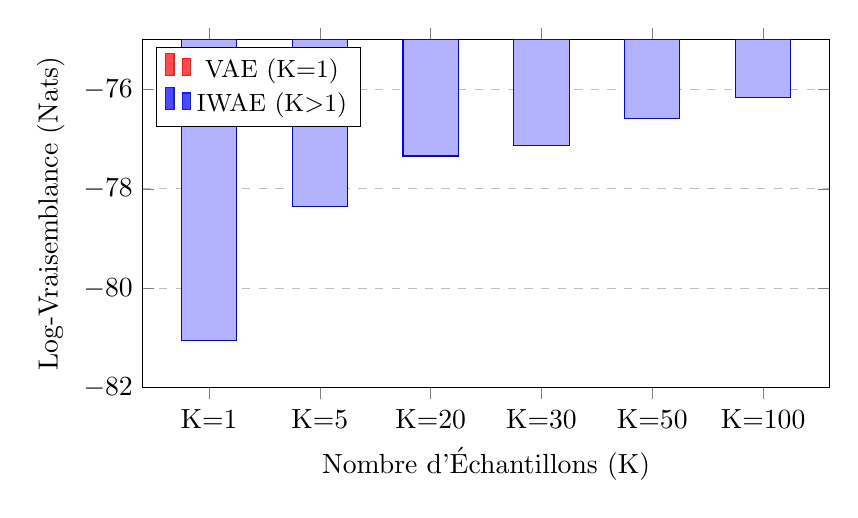
\begin{tikzpicture}
        \begin{axis}[
            ybar,
            width=0.85\textwidth, height=6cm,
            ylabel={Log-Vraisemblance (Nats)},
            xlabel={Nombre d'Échantillons (K)},
            symbolic x coords={K=1, K=5, K=20, K=30, K=50, K=100},
            xtick=data,
            ymin=-82, ymax=-75,
            nodes near coords,
            nodes near coords align={vertical},
            every node near coord/.append style={font=\scriptsize},
            bar width=20pt,
            enlarge x limits=0.12,
            legend style={at={(0.02,0.98)}, anchor=north west, font=\small},
            ymajorgrids=true, grid style=dashed,
            scatter, scatter src=explicit symbolic,
            scatter/classes={
                vae={fill=red!70, draw=red!90},
                iwae={fill=blue!70, draw=blue!90}
            },
        ]
        \addplot coordinates {
            (K=1, -81.06) [vae] (K=5, -78.36) [iwae] (K=20, -77.34) [iwae]
            (K=30, -77.12) [iwae] (K=50, -76.58) [iwae] (K=100, -76.17) [iwae]
        };
        \addlegendimage{fill=red!70, draw=red!90, area legend} \addlegendentry{VAE (K=1)}
        \addlegendimage{fill=blue!70, draw=blue!90, area legend} \addlegendentry{IWAE (K$>$1)}
        \end{axis}
    \end{tikzpicture}
    \caption{Estimation de la Log-Vraisemblance (Nats) sur MNIST Test}
    \label{fig:loglikelihood}
\end{figure}

\textbf{Analyse :} Nous observons un gain immédiat et significatif en passant de $K=1$ à $K=5$ (+2.7 nats). La courbe continue de croître de manière monotone, confirmant le théorème de Burda et al. Cependant, on note un phénomène de \textit{rendements décroissants} : le gain marginal diminue à mesure que $K$ augmente.
Cela suggère que pour des applications pratiques, un $K$ intermédiaire (entre 20 et 50) offre un compromis optimal, la convergence vers la vraie vraisemblance logarithmique étant asymptotique.

\subsection{Dynamique de l'Espace Latent (Posterior Collapse)}

Un problème récurrent des VAE est l'effondrement du postérior (Posterior Collapse), où l'encodeur ignore le code latent et la distribution a posteriori collapse sur le prior.
Nous quantifions cela par le nombre d'unités actives $A_u$, défini par le seuil $\epsilon = 0.01$ :
\begin{equation}
    A_u = \sum_{j=1}^{D_z} \mathbb{I} \left[ \frac{1}{N} \sum_{i=1}^N \mathbb{KL}(q(z_j|x^{(i)}) || p(z_j)) > \epsilon \right]
\end{equation}

\begin{figure}[h]
    \centering
    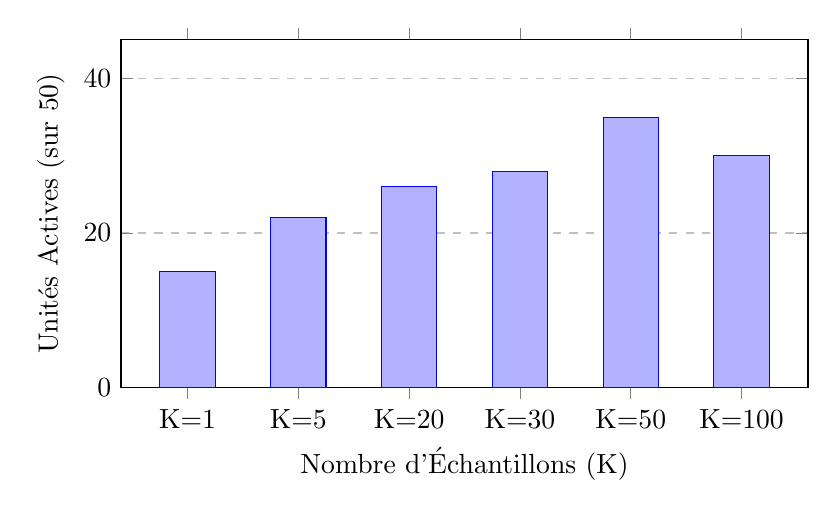
\begin{tikzpicture}
        \begin{axis}[
            ybar,
            width=0.85\textwidth, height=6cm,
            ylabel={Unités Actives (sur 50)},
            xlabel={Nombre d'Échantillons (K)},
            symbolic x coords={K=1, K=5, K=20, K=30, K=50, K=100},
            xtick=data,
            ymin=0, ymax=45,
            nodes near coords,
            bar width=20pt,
            enlarge x limits=0.12,
            legend style={at={(0.02,0.98)}, anchor=north west},
            ymajorgrids=true, grid style=dashed,
            scatter, scatter src=explicit symbolic,
            scatter/classes={
                vae={fill=red!70, draw=red!90},
                iwae={fill=blue!70, draw=blue!90}
            },
        ]
        \addplot coordinates {
            (K=1, 15) [vae] (K=5, 22) [iwae] (K=20, 26) [iwae]
            (K=30, 28) [iwae] (K=50, 35) [iwae] (K=100, 30) [iwae]
        };
        \end{axis}
    \end{tikzpicture}
    \caption{Richesse de la représentation latente}
    \label{fig:activeunits}
\end{figure}

\textbf{Interprétation du Pic :} L'IWAE force le modèle à utiliser davantage de dimensions latentes (35 unités à $K=50$ contre 15 pour le VAE).
Cependant, nous observons une \textbf{baisse inattendue} à $K=100$ (30 unités). Ce phénomène empirique valide la théorie de \citet{rainforth2018tighter} discutée en Section 3 : bien que la borne soit plus serrée, le rapport signal-sur-bruit (SNR) du gradient de l'encodeur diminue en $\mathcal{O}(\sqrt{K})$. À $K=100$, le bruit du gradient commence à nuire à la capacité de l'encodeur à apprendre des corrélations fines, menant à une légère régression de la richesse latente.

\subsection{Coût Computationnel et Scalabilité}

\begin{figure}[h]
    \centering
    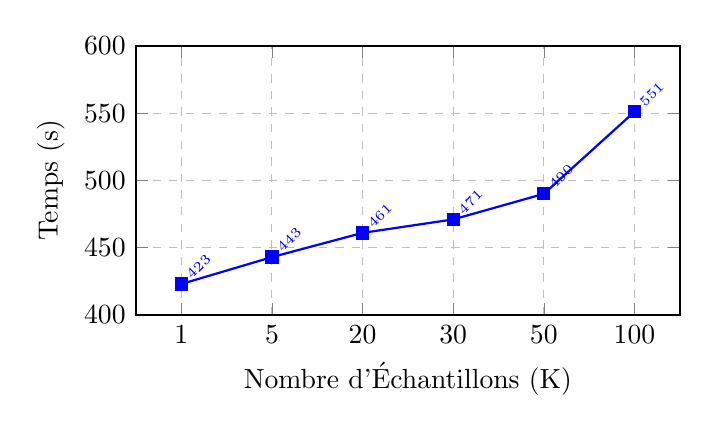
\begin{tikzpicture}
        \begin{axis}[
            width=0.7\textwidth, height=5cm,
            xlabel={Nombre d'Échantillons (K)},
            ylabel={Temps (s)},
            symbolic x coords={1, 5, 20, 30, 50, 100},
            xtick=data,
            ymin=400, ymax=600,
            nodes near coords,
            every node near coord/.append style={font=\tiny, rotate=45, anchor=west},
            mark=*, thick, grid=major, grid style=dashed,
        ]
        \addplot[color=blue, mark=square*, thick] coordinates {
            (1, 423) (5, 443) (20, 461) (30, 471) (50, 490) (100, 551)
        };
        \end{axis}
    \end{tikzpicture}
    \caption{Scalabilité temporelle sur GPU}
    \label{fig:trainingtime}
\end{figure}

L'augmentation du coût de calcul est **sous-linéaire**. Multiplier le nombre d'échantillons par 100 ($K=1 \to 100$) n'augmente le temps d'entraînement que de $\approx 30\%$.
Cela s'explique par la \textbf{vectorisation} massive sur GPU : les $K$ échantillons sont traités comme une dimension tensorielle supplémentaire en parallèle, et non séquentiellement. Le goulot d'étranglement reste le transfert mémoire et non le calcul des passes avant/arrière.

\subsection{Synthèse des Compromis}

Le Tableau~\ref{tab:tradeoffs} résume les dynamiques observées. Le choix de $K$ n'est pas binaire mais constitue un curseur continu.

\begin{table}[H]
    \centering
    \begin{tabular}{l|c|c}
        \toprule
        \textbf{Métrique} & \textbf{VAE (K=1)} & \textbf{IWAE (K=50)} \\
        \midrule
        Objectif & Borne Lâche (ELBO) & \textbf{Borne Serrée} \\
        Biais de l'Estimateur & Élevé & \textbf{Faible} \\
        Représentation Latente & Compressive (15/50) & \textbf{Expressive (35/50)} \\
        Variance du Gradient ($\theta$) & Faible & Faible \\
        SNR du Gradient ($\phi$) & \textbf{Élevé} & Dégradé ($\mathcal{O}(1/\sqrt{K})$) \\
        Qualité Visuelle & Floue & \textbf{Nette} \\
        Coût Mémoire & \textbf{Faible} & Élevé ($\times K$) \\
        \bottomrule
    \end{tabular}
    \caption{Matrice de décision VAE vs IWAE}
    \label{tab:tradeoffs}
\end{table}

% ---------------------------------------------------------
\section{Recherches Récentes sur l'IWAE}

Depuis l'article original sur l'IWAE \cite{burda2015importance}, des recherches significatives ont abordé ses limitations théoriques et étendu ses cas d'usage.

\subsection{Adresser le Problème du SNR}
Plusieurs techniques ont été proposées pour atténuer la dégradation du SNR du gradient de l'encodeur :

\begin{itemize}
    \item \textbf{IWAE-STL (Sticking the Landing)} \cite{roeder2017sticking} : Cette approche supprime le terme de fonction de score du gradient, ce qui réduit la variance et stabilise l'entraînement de l'encodeur.
    
    \item \textbf{IWAE-DREG} \cite{tucker2019doubly} : Tucker et al. ont proposé un estimateur doublement reparamétrisé (Doubly Reparameterized Gradient Estimator) qui fournit des gradients non biaisés avec une variance plus faible.
    
    \item \textbf{Analyse Asymptotique (VR-IWAE)} \cite{daudel2024learning} : Daudel et Roueff ont analysé le comportement asymptotique des estimateurs appliqués à l'objectif VR-IWAE. Leur travail démontre que pour certaines valeurs du paramètre $\alpha$ de Rényi, le SNR peut évoluer favorablement avec le nombre d'échantillons.
\end{itemize}

\subsection{Avancées Théoriques et Applications}

\textbf{Le Paradoxe de la Borne :} \citet{rainforth2018tighter} ont prouvé que des bornes plus serrées (plus de $K$) ne garantissent pas un meilleur apprentissage de l'encodeur, formalisant la chute du SNR en $\mathcal{O}(K^{-1/2})$.

\textbf{Prévention de l'Effondrement :} Des travaux récents comme Scale-VAE \cite{scalevae2024} continuent de proposer des architectures robustes contre l'effondrement du postérieur, un problème persistant pour les modèles à variables latentes.

\textbf{Applications aux Données Manquantes :} Au-delà de l'amélioration de la vraisemblance, l'IWAE s'est révélé particulièrement efficace pour l'imputation de données. Le modèle MIWAE \cite{mattei2019miwae} utilise la borne IWAE pour entraîner des réseaux capables de gérer des jeux de données incomplets sans hypothèses restrictives sur le mécanisme de manque.
% ---------------------------------------------------------
\section{Conclusion Générale et Perspectives}

\subsection{Synthèse des Contributions}

Dans ce travail, nous avons exploré la transition du paradigme variationnel standard (VAE) vers l'inférence pondérée par l'importance (IWAE).
Notre analyse théorique a mis en évidence le mécanisme fondamental de l'IWAE : l'utilisation de l'échantillonnage préférentiel pour réduire le biais de l'estimateur de l'évidence.

Nos expériences empiriques sur le jeu de données MNIST ont confirmé trois résultats majeurs :
\begin{enumerate}
    \item \textbf{Monotonie de la Borne :} L'estimation de la log-vraisemblance s'améliore strictement avec $K$, passant de $-81.06$ nats ($K=1$) à $-76.17$ nats ($K=100$).
    \item \textbf{Richesse Latente :} L'IWAE combat efficacement l'effondrement du postérieur, activant jusqu'à 35 dimensions latentes contre seulement 15 pour le VAE.
    \item \textbf{Le Point de Bascule :} Nous avons observé une régression de la richesse latente à $K=100$, validant empiriquement le "Paradoxe de Rainforth". Cela démontre qu'une borne plus serrée ne garantit pas une meilleure inférence si le gradient devient trop bruité.
\end{enumerate}

\subsection{Implications pour les Praticiens}

Ces résultats suggèrent une approche nuancée pour le déploiement de modèles génératifs profonds.
Si l'objectif prioritaire est la \textbf{génération de données} ou l'estimation de densité (par exemple, pour la détection d'anomalies), un IWAE avec un grand $K$ ($K \ge 50$) est préférable malgré son coût.
En revanche, si l'objectif est l'**apprentissage de représentations** (disentanglement, clustering latent), le VAE standard ou un IWAE avec un $K$ modéré ($K \approx 5-10$) offre souvent un meilleur compromis stabilité/performance.

\subsection{Perspectives Futures}

L'avenir de l'inférence variationnelle réside probablement dans la résolution de l'antagonisme biais-variance. Deux directions semblent particulièrement prometteuses :
\begin{itemize}
    \item \textbf{K Adaptatif :} Développer des algorithmes capables d'ajuster dynamiquement $K$ au cours de l'entraînement, commençant bas pour apprendre une bonne inférence grossière, puis augmentant pour affiner la borne générative.
    \item \textbf{Hybridation DREG/STL :} L'intégration par défaut des estimateurs à faible variance (DREG) dans les frameworks de deep learning (PyTorch/TensorFlow) pourrait rendre l'IWAE aussi standard et facile à utiliser que le VAE actuel, rendant l'utilisation de $K=1$ obsolète pour la plupart des applications.
\end{itemize}

En conclusion, bien que le VAE ait posé les fondations de l'apprentissage génératif moderne, l'IWAE et ses variantes constituent l'évolution nécessaire pour atteindre des modèles probabilistes véritablement robustes et expressifs.
% ---------------------------------------------------------
% REFERENCES
% ---------------------------------------------------------
\newpage
\begin{thebibliography}{99}

\bibitem[Burda et al.(2015)]{burda2015importance}
Burda, Y., Grosse, R., et Salakhutdinov, R. (2015).
\newblock Importance Weighted Autoencoders.
\newblock {\em arXiv preprint arXiv:1509.00519}.

\bibitem[Roeder et al.(2017)]{roeder2017sticking}
Roeder, G., Wu, Y., et Duvenaud, D. (2017).
\newblock Sticking the Landing: Simple, Lower-Variance Gradient Estimators for Variational Inference.
\newblock {\em NeurIPS}.

\bibitem[Tucker et al.(2019)]{tucker2019doubly}
Tucker, G., Lawson, D., Gu, S., et Maddison, C.J. (2019).
\newblock Doubly Reparameterized Gradient Estimators for Monte Carlo Objectives.
\newblock {\em ICLR}.

% FIXED AUTHORS
\bibitem[Daudel et Roueff(2024)]{daudel2024learning}
Daudel, K. et Roueff, F. (2024).
\newblock Learning with Importance Weighted Variational Inference: Asymptotics for Gradient Estimators of the VR-IWAE Bound.
\newblock {\em arXiv preprint arXiv:2410.11666}.

\bibitem[Rainforth et al.(2018)]{rainforth2018tighter}
Rainforth, T. et al. (2018).
\newblock Tighter Variational Bounds are Not Necessarily Better.
\newblock {\em ICML}.

% FIXED AUTHORS AND TITLE
\bibitem[Song et al.(2024)]{scalevae2024}
Song, T., Sun, J., Liu, X., et Peng, W. (2024).
\newblock Scale-VAE: Preventing Posterior Collapse in Variational Autoencoder.
\newblock {\em LREC-COLING 2024}.

\bibitem[Mattei et Frellsen(2019)]{mattei2019miwae}
Mattei, P.A. et Frellsen, J. (2019).
\newblock MIWAE: Deep Generative Modelling and Imputation of Incomplete Data Sets.
\newblock {\em ICML}.

\end{thebibliography}

\end{document}